\section{Results}
\label{sec:results}

\subsection{Shuffled Negatives Benchmark (132 TFs)}

Table~\ref{tab:main_shuf} summarizes performance on the full 132-TF benchmark with dinucleotide-shuffled negatives.

\begin{table}[H]
\centering
\caption{Benchmark results on 132 ENCODE K562 ChIP-seq datasets (shuffled negatives).}
\label{tab:main_shuf}
\small
\begin{tabular}{lrrr}
\toprule
Tool & Mean AUROC & Time/TF & Speedup vs.\ STREME \\
\midrule
\textbf{motif-discover}    & \textbf{0.842} & \textbf{0.30\,s} & \textbf{11$\times$} \\
proto-motif-discover       & 0.843 & 1.56\,s & 2.1$\times$ \\
STREME 5.5.5               & 0.803 & 3.26\,s & 1.0$\times$ \\
\bottomrule
\end{tabular}
\end{table}

motif-discover significantly outperforms STREME ($\Delta = +0.039$ AUROC, Wilcoxon $p = 4.1 \times 10^{-7}$, 85 wins / 43 losses / 4 ties). The improvement is consistent across TF families and is not driven by a few outliers (bootstrap 95\% CI of $\Delta$: [0.023, 0.046]).

\begin{figure}[H]
\centering
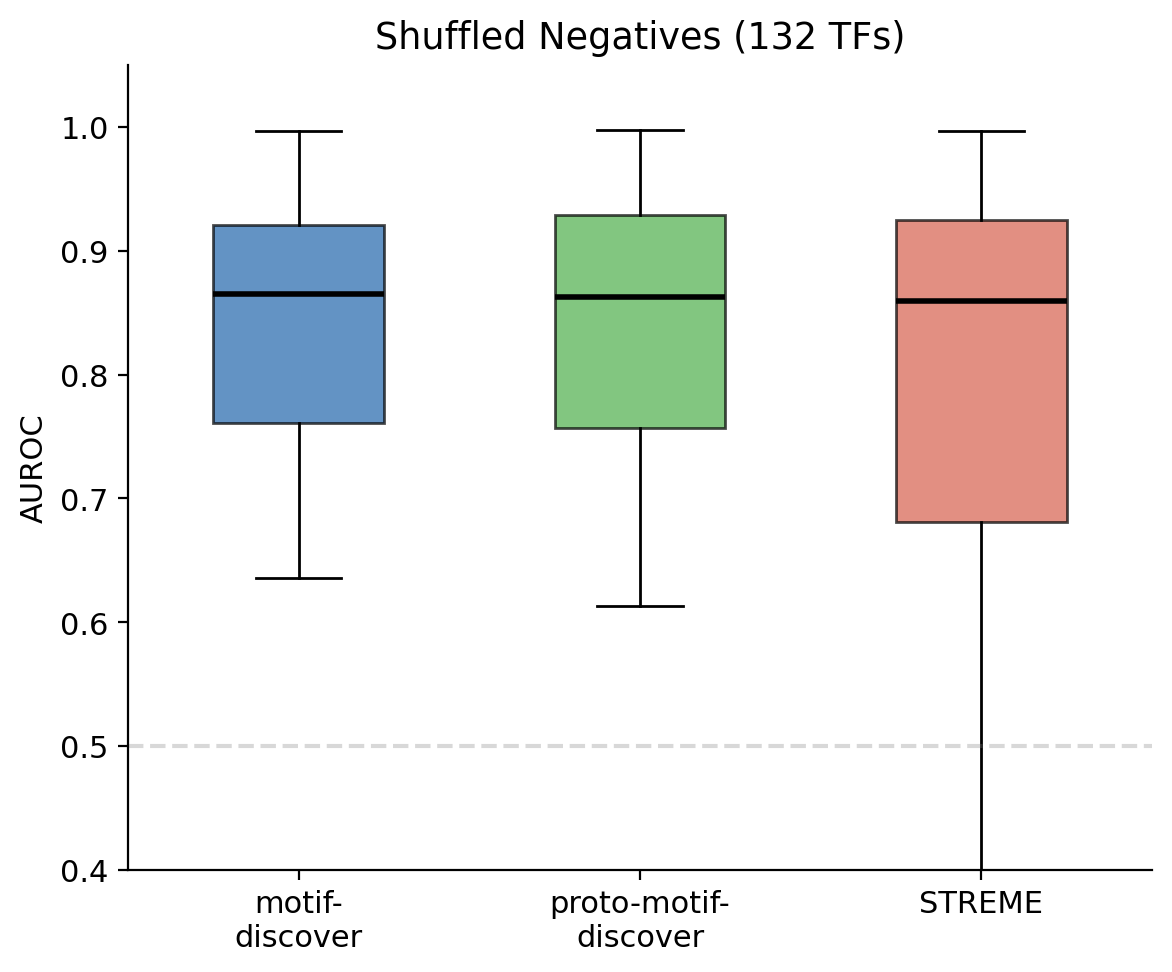
\includegraphics[width=0.7\textwidth]{figures/fig1_auroc_boxplot}
\caption{AUROC distribution across 132 ENCODE K562 ChIP-seq datasets (shuffled negatives). motif-discover consistently outperforms STREME. Dashed line indicates random performance.}
\label{fig:boxplot}
\end{figure}

\begin{figure}[H]
\centering
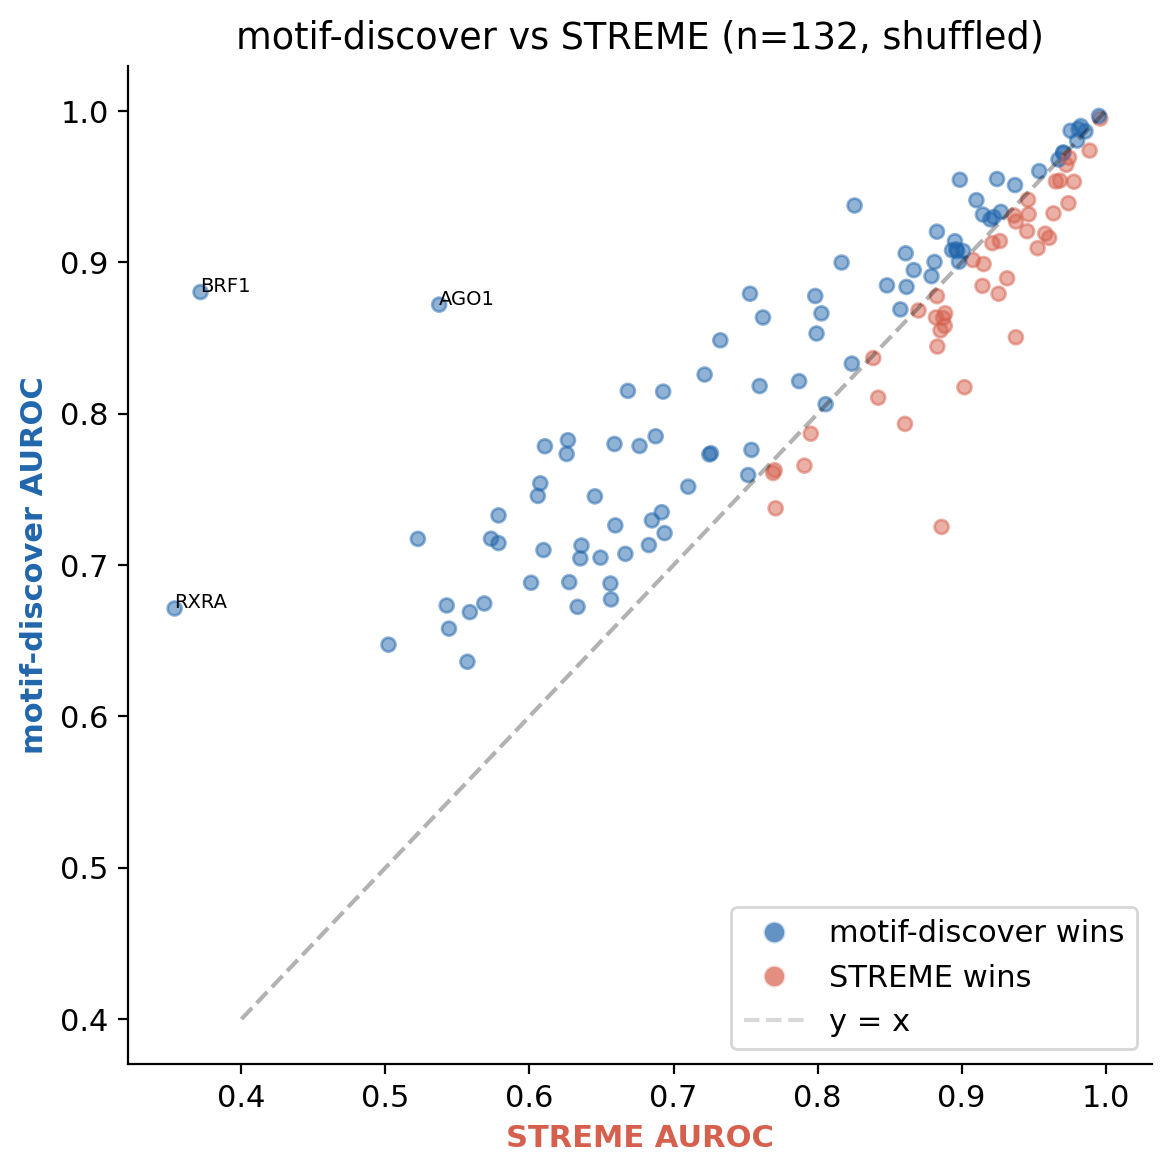
\includegraphics[width=0.6\textwidth]{figures/fig2_scatter_shuffled}
\caption{Per-TF comparison: motif-discover vs.\ STREME (132 TFs, shuffled negatives). Points above the diagonal indicate TFs where motif-discover outperforms STREME.}
\label{fig:scatter_shuf}
\end{figure}

\subsection{Genomic Negatives Benchmark}

On the more realistic benchmark using hg38 genomic regions as negatives with Markov-1 background scoring, motif-discover was evaluated on two subsets:

\paragraph{132-TF genomic (motif-discover vs.\ proto-motif-discover).}
On the full 132-TF set, motif-discover achieves 0.896 AUROC versus proto's 0.856 ($\Delta = +0.040$, Wilcoxon $p = 1.7 \times 10^{-14}$, 101 wins / 22 losses). This confirms that the current version represents a substantial improvement over the earlier prototype on realistic genomic DNA.

\paragraph{53-TF genomic (full comparison).}
On the 53-TF subset where STREME and MEME genomic results are also available:

\begin{table}[H]
\centering
\caption{Genomic negatives benchmark (53 TFs, Markov-1 scoring).}
\label{tab:main_gen}
\small
\begin{tabular}{lrr}
\toprule
Tool & Mean AUROC & Time/TF \\
\midrule
\textbf{motif-discover}    & \textbf{0.891} & \textbf{0.3\,s} \\
MEME 5.5.5                 & 0.881 & $\sim$90\,s \\
proto-motif-discover       & 0.874 & 1.4\,s \\
STREME 5.5.5               & 0.863 & 4.4\,s \\
\bottomrule
\end{tabular}
\end{table}

motif-discover outperforms STREME by $+0.028$ AUROC (Wilcoxon $p = 6.5 \times 10^{-4}$, 35 wins / 16 losses) while running \textbf{15$\times$ faster} (0.3\,s vs.\ 4.4\,s per TF). It also edges out MEME by $+0.010$ AUROC while running approximately \textbf{300$\times$ faster}.

\begin{figure}[H]
\centering
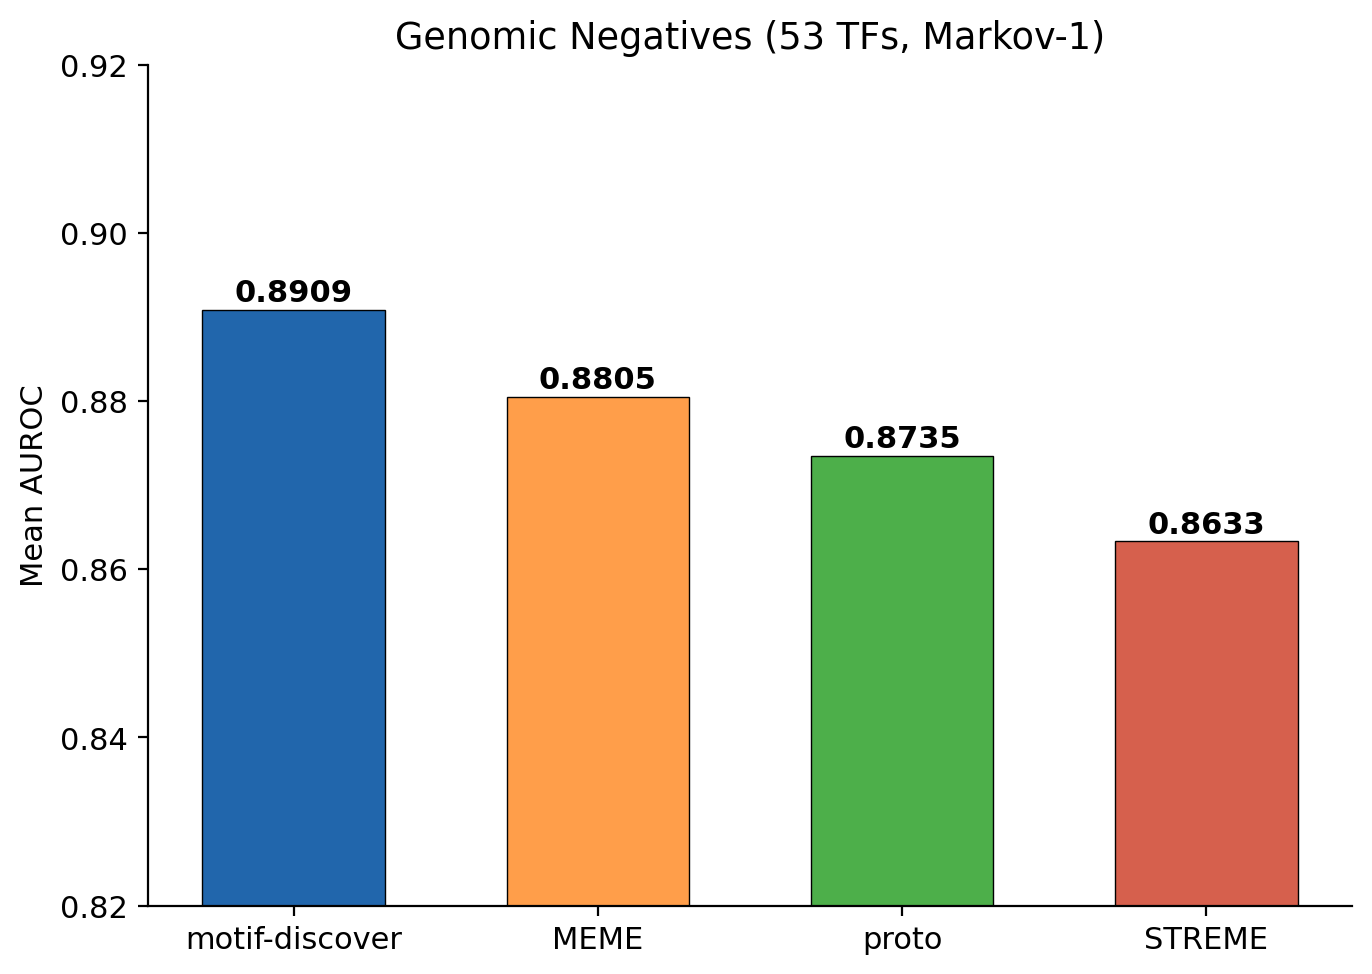
\includegraphics[width=0.65\textwidth]{figures/fig4_genomic_comparison}
\caption{Genomic negatives benchmark (53 TFs, Markov-1 scoring). motif-discover outperforms all three comparison tools.}
\label{fig:genomic}
\end{figure}

\begin{figure}[H]
\centering
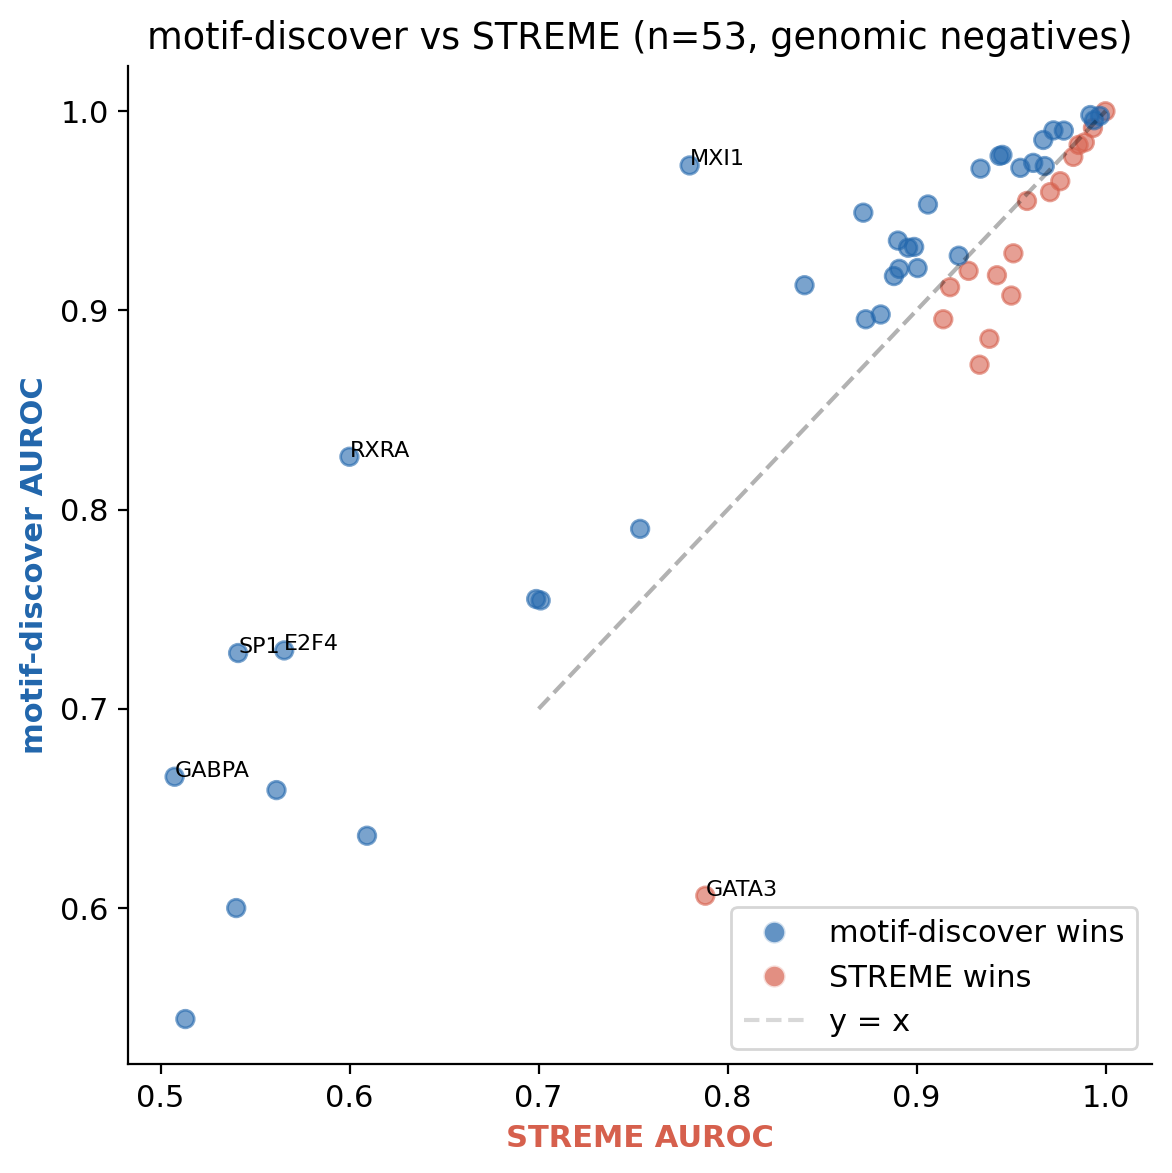
\includegraphics[width=0.6\textwidth]{figures/fig5_scatter_genomic}
\caption{Per-TF comparison: motif-discover vs.\ STREME (53 TFs, genomic negatives). Points above the diagonal indicate TFs where motif-discover outperforms STREME.}
\label{fig:scatter_gen}
\end{figure}

\subsection{Speed}

The speed advantage is substantial across all benchmarks:

\begin{figure}[H]
\centering
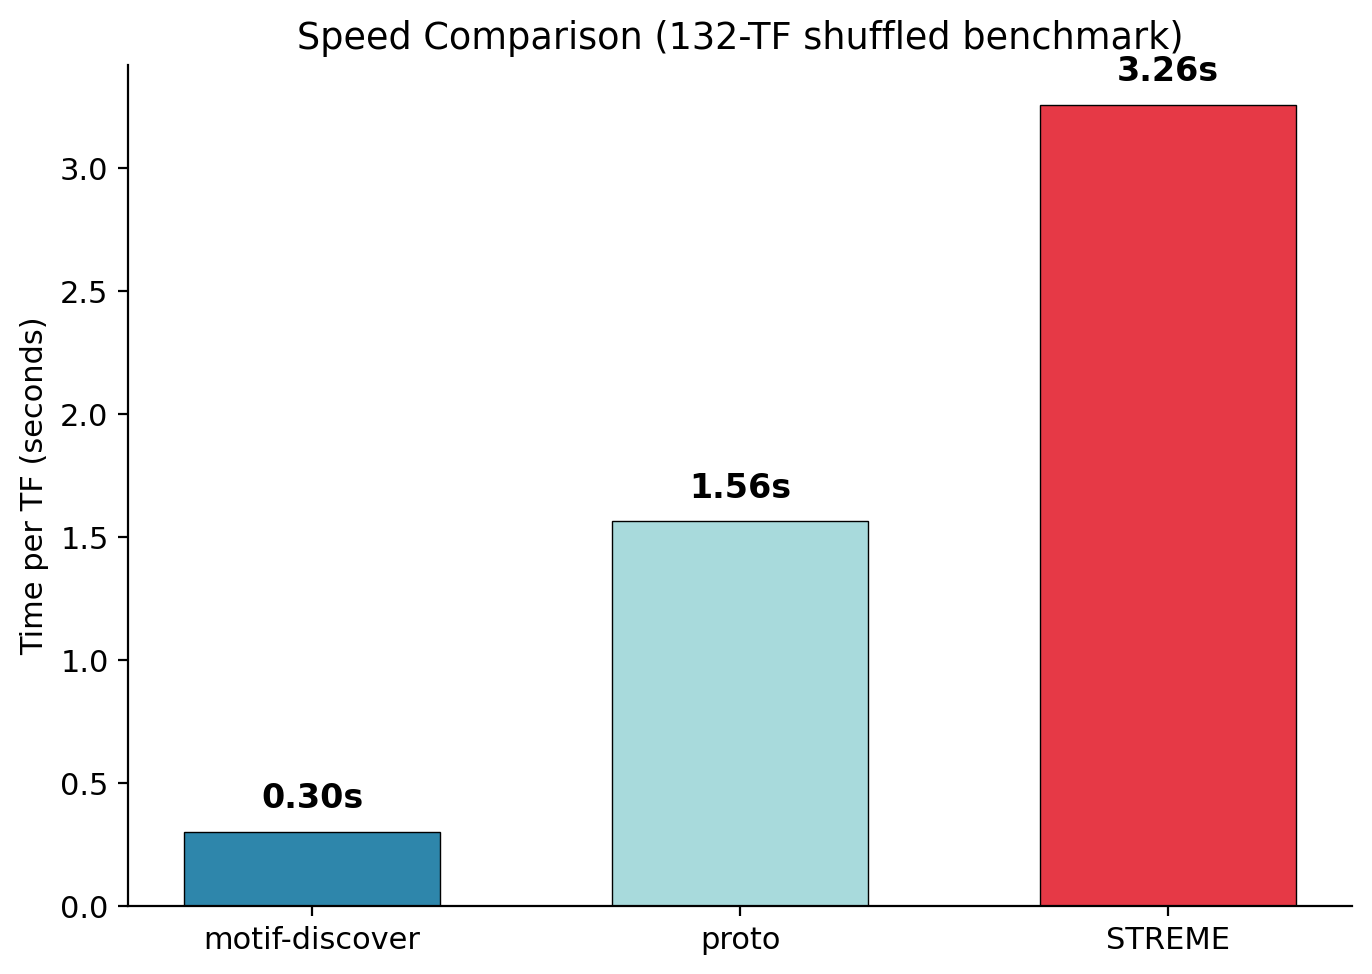
\includegraphics[width=0.65\textwidth]{figures/fig3_speed_comparison}
\caption{Runtime per TF across tools (132-TF shuffled benchmark). motif-discover processes all 132 TFs in under 45 seconds.}
\label{fig:speed}
\end{figure}

At 0.3\,s per TF, motif-discover processes the full 132-TF benchmark in under 45 seconds. STREME requires approximately 7 minutes. MEME requires approximately 3 hours. The speedup is algorithmic --- all tools were compiled with identical optimization flags and run on identical hardware.

\subsection{Per-TF Analysis}

motif-discover wins 85 of 132 TFs against STREME on shuffled negatives. The largest individual improvements include TFs where STREME struggles with short or degenerate motifs (e.g., AGO1: $+0.31$, BRF1: $+0.26$, RXRA: $+0.23$). STREME's wins tend to occur on TFs where its default width range captures wider binding patterns (e.g., BDP1: $-0.11$, CEBPG: $-0.09$); motif-discover supports configurable width ranges to address such cases.

\subsection{Statistical Significance}

The improvement over STREME is robust across multiple tests:

\begin{table}[H]
\centering
\caption{Statistical significance of motif-discover vs.\ STREME.}
\label{tab:stats}
\small
\begin{tabular}{lrr}
\toprule
Test & Shuffled (132 TFs) & Genomic (53 TFs) \\
\midrule
Wilcoxon $p$         & $4.1 \times 10^{-7}$ & $6.5 \times 10^{-4}$ \\
Bootstrap 95\% CI    & [0.023, 0.046]       & [0.010, 0.046] \\
McNemar $\chi^2$     & 13.1 ($p = 2.9 \times 10^{-4}$) & 6.4 ($p = 1.2 \times 10^{-2}$) \\
Cliff's $\delta$     & $+0.31$              & $+0.38$ \\
Cohen's $d$ (paired) & $+0.48$              & $+0.42$ \\
Wins / Losses        & 85 / 43              & 35 / 16 \\
\bottomrule
\end{tabular}
\end{table}

\subsection{Biological Validity}

TOMTOM analysis (version 5.5.5, Pearson distance) against the JASPAR 2026 Core database (2{,}633 motifs) confirmed that discovered motifs are biologically meaningful. Table~\ref{tab:tomtom} summarizes the results.

\begin{table}[H]
\centering
\caption{TOMTOM JASPAR match summary ($n = 119$ TFs with motifs tested).}
\label{tab:tomtom}
\small
\begin{tabular}{lrr}
\toprule
Metric & motif-discover & STREME \\
\midrule
Any JASPAR match            & 112 (94\%) & 104 (87\%) \\
Significant ($e < 0.05$)    & 93 (78\%)  & 88 (74\%) \\
Strong match ($e < 0.001$)  & 55 (46\%)  & 51 (43\%) \\
Median best e-value         & $1.6 \times 10^{-3}$ & $1.1 \times 10^{-3}$ \\
Top-5 moderate ($q < 0.05$) & 100\% & 100\% \\
Top-1 strict ($q < 0.001$, $\geq$70\% overlap) & 50\% & 62\% \\
Better e-value head-to-head & 52 / 97 & 45 / 97 \\
\bottomrule
\end{tabular}
\end{table}

Both tools achieve 100\% top-5 moderate match rate: every TF has at least one discovered motif matching a known JASPAR entry. motif-discover actually matches more TFs overall (94\% vs.\ 87\%) and wins the head-to-head e-value comparison (52 vs.\ 45). STREME's higher strict match rate (62\% vs.\ 50\%) reflects its tendency to discover wider motifs that achieve higher overlap fractions with JASPAR references — a width artifact rather than a correctness difference.

\subsection{Memory Usage}

motif-discover uses 10\,MB peak RSS across all TFs. STREME uses approximately 113\,MB per TF. The minimal footprint enables deployment in resource-constrained environments such as containerized pipelines or cloud functions.
